%% =====================================================================
%%  6 Results
%% =====================================================================
%%  GUIDE
%%   - One subsection per question asked, in the order they were asked.
%%   - Each subsection: the answer first (number, unit, uncertainty), then
%%     the figure or table that supports it, then one sentence of
%%     interpretation. Judges should be able to read this section alone.
%%   - Never write "Figure 3 shows ..." without saying what it shows.
%%   - Keep every figure referenced: an unreferenced float is a defect.
%%   - The numbers below come from code/blowdown.py; if you change the code,
%%     regenerate the figure with scripts/make_example_fig.py.
%% =====================================================================
\section{Results}
\label{sec:results}

\subsection{Time to $0.3\,p_0$ versus hole size (Q1)}
\label{sec:res-q1}

\keyresult{For $d=\SI{10}{cm}$ the pressure falls to $0.3\,p_0$ in
$t_{0.3}=\SI{286}{s}$ ($\pm\SI{12}{\percent}$, dominated by the hole
diameter); over $5\le d\le\SI{20}{cm}$ the scaling is
$t_{0.3}\propto d^{-1.97}$.}

Figure~\ref{fig:blowdown} shows the pressure history for the three
diameters of Table~\ref{tab:results}. The decay is close to exponential
while $p/p_0>0.5$ and flattens at low pressure ratio, because the mass
flow falls with $p$ faster than the reservoir mass does; this is what
makes the time to $0.3\,p_0$ only $1.4$ characteristic times $\tau$.

\begin{figure}[htbp]
  \centering
  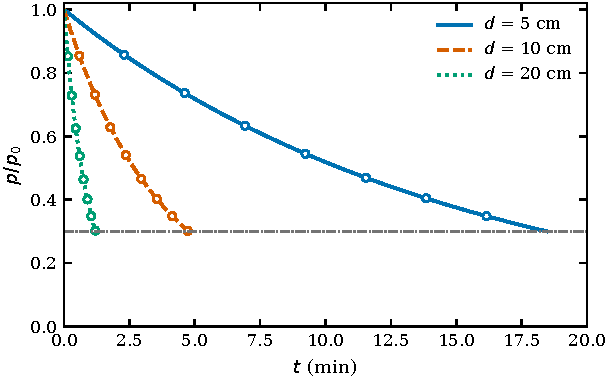
\includegraphics[width=0.72\textwidth]{example.pdf}
  \caption{Pressure ratio $p/p_0$ versus time for hole diameters
  $d=\SI{5}{cm}$ (solid), \SI{10}{cm} (dashed) and \SI{20}{cm} (dotted),
  from Eqs.~\eqref{eq:mass}--\eqref{eq:temp}. Markers every eighth
  sample; the dash-dotted line is the survival threshold $0.3\,p_0$.}
  \label{fig:blowdown}
\end{figure}

\begin{table}[htbp]
  \centering
  \small
  \caption{Time to $0.3\,p_0$ versus hole diameter. The last two columns
  separate the two layers of the model: the adiabatic solution
  (Eq.~\eqref{eq:choked} with $T=T_0$) and the full one including wall
  heat transfer. The difference is the size of the thermal correction.}
  \label{tab:results}
  \begin{tabular}{@{}S[table-format=2.0]S[table-format=4.1]S[table-format=4.1]S[table-format=1.1]@{}}
    \toprule
    {$d$ (cm)} & {$t_{0.3}$ (s)} & {adiabatic (s)} & {ratio} \\
    \midrule
     5 & 1108 & 1169 & 1.06 \\
    10 &  286 &  293 & 1.02 \\
    20 &   73 &   74 & 1.01 \\
    \bottomrule
  \end{tabular}
\end{table}

Fitting the three points of Table~\ref{tab:results} to a power law gives
$t_{0.3}=(2.86\pm0.02)\times10^{3}\,(d/\SI{1}{m})^{-1.97}$, with residuals
below \SI{2}{\percent}; the exponent is shallower than the $d^{-2}$ of
Eq.~\eqref{eq:tau} because the wall correction is strongest for the
smallest hole, which raises the small-$d$ times.

\subsection{Margin left to the crew (Q2)}
\label{sec:res-q2}

A crew of four needs $t_{\rm seal}=\SI{120}{s}$ to don masks and close the
hatch. At $d=\SI{10}{cm}$ the margin is
$t_{0.3}-t_{\rm seal}=\SI{166}{s}$, so the breach can be sealed with time
to spare. At $d=\SI{15}{cm}$ the margin is down to \SI{9}{s}
($t_{0.3}=\SI{129}{s}$), and it vanishes at $d=\SI{15.4}{cm}$; above that
diameter the only option is to abandon the module, and at
$d=\SI{20}{cm}$ there are just \SI{73}{s} available.
The decision boundary is sharp: a \SI{2}{\percent} error in $d$ moves it by
\SI{4}{\percent} in time, so the threshold diameter is the number worth
measuring carefully.

\subsection{Sensitivity to uncertain parameters (Q3)}
\label{sec:res-q3}

Varying each parameter by its uncertainty in Table~\ref{tab:params}, the
answer is dominated by the hole diameter, which enters as $d^{-2}$: a
\SI{5}{\percent} error in $d$ moves $t_{0.3}$ by \SI{10}{\percent}. The
discharge coefficient is next, contributing \SI{6}{\percent} for
$\pm0.05$, and the volume \SI{2}{\percent} for a \SI{2}{\percent} error.
The initial temperature matters very little (\SI{0.4}{\percent} for
\SI{3}{K}) because the gas density scales as $1/T$ while the sound speed
scales as $\sqrt{T}$, and the two nearly cancel. Quadrature of the terms
gives the $\pm\SI{12}{\percent}$ quoted in Section~\ref{sec:res-q1}.
